\section{Data Analysis}
\label{sec:Analysis}
In this work we re-analyze  scientific run~II data recorded between February 2011 and March 2012, 
corresponding to 224.6~live~days. The characterization of the detector response to ER interactions is performed using dedicated calibration campaigns with $^{60}$Co and $^{232}$Th radioactive sources, while the response to NR interactions is preformed using $^{241}$AmBe calibration campaigns.
%\sout{as well as for estimating the background from $\beta$ and $\gamma$-particles. For the ER sample we expose the detector to $^{60}$Co and $^{232}$Th sources, while for the NR sample we use $^{241}$AmBe.}

 
This work extends the previous results~\cite{xe100_run10_si,xe100_run_combination}, referred to in the following as the low energy channel, with a new study exploring the energy range between 43-240\,keV. 
The data analysis is divided into two mutually exclusive channels, one optimized for low energies and ranging from 3-30\,PE in cS1 (lowE), 
the other optimized for high energies recoils ranging from 30-180\,PE in cS1 (highE).  These two analysis are finally statistically combined. 
The relative region of interests (ROI) of these two channels are shown in Figure~\ref{fig:phasespace} and further described in the following sections. 


\subsection{Low Energy Channel}
\label{subsec:LowE}
This analysis channel relies on the re-analysis of run~II data described in~\cite{xe100_run_combination}. The region of interest (ROI), the background 
expectation models, data selections and their acceptances are mostly unchanged and so are only briefly summarized here. Differences with respect to said results are highlighted when present.

The ROI for this channel is defined in the ($y,cS1$)-plane and is shown in Figure~\ref{fig:phasespace}.  The lower 
bound on $y$ corresponds to a 3\,$\sigma$ acceptance quantile (as a function of cS1) of a 20~GeV WIMP mass signal model assuming an $\mathcal{O}_1$ (SI) interaction, while the upper bound is fixed at y\,=\,2.7.
The range in cS1 is selected as 3 to 30\,PE. 
The ROI is further divided into eight sub-regions (also called bands) depending on the operator $\mathcal{O}_i$ and on the WIMP mass hypothesis. 
These bands are arranged to achieve constant expected signal density in each region, as described in~\cite{xe100_run_combination}.

\begin{figure}[]
\begin{minipage}{1\linewidth}
\centerline{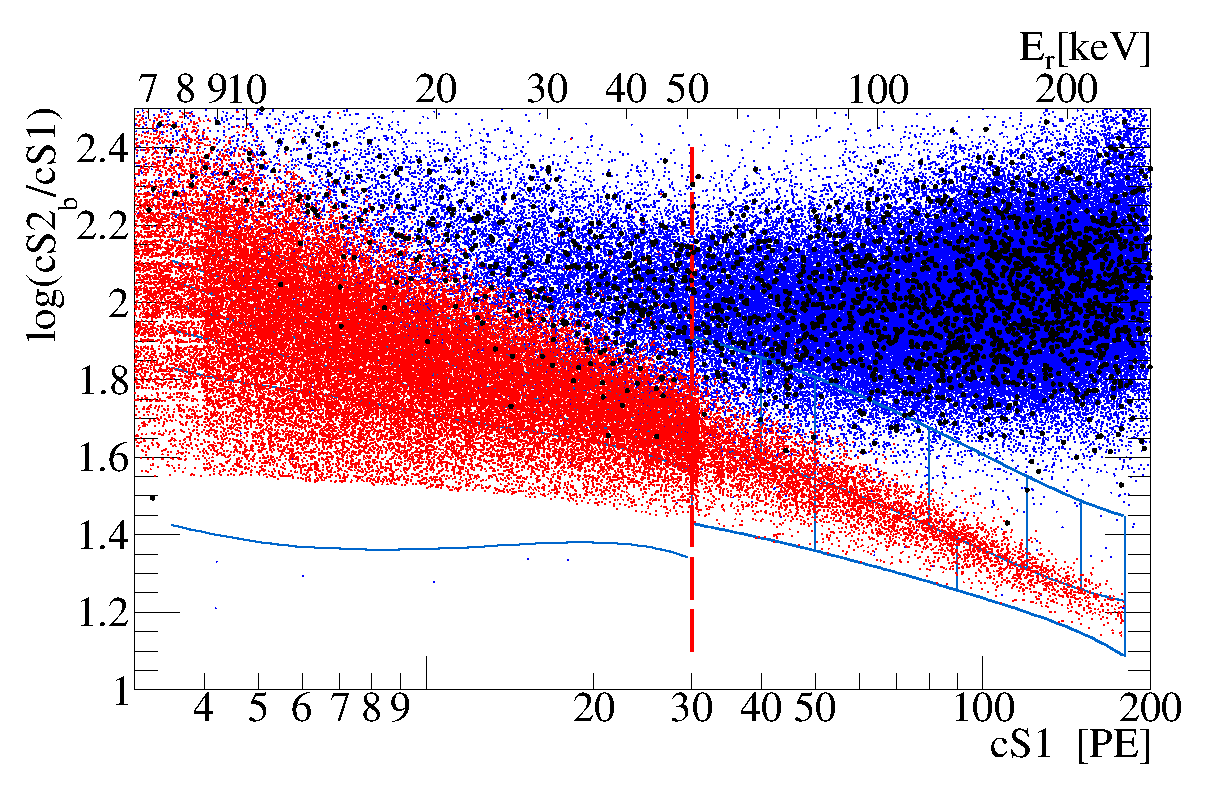
\includegraphics[width=1\linewidth]{Figures/eft_sr.eps}}
\end{minipage}
\caption{Summary of regions of interest, backgrounds, and observed data. ER calibration data, namely $^{60}\mathrm{Co}$ and $^{232}\mathrm{Th}$ data is shown as blue dots. NR calibration data ($^{241}$AmBe) is shown as red dots. Dark matter search data is shown as black dots. The red dashed line is the threshold between the low and high energy channels. The lines in blue are the bands. For the low-energy channel these are operator and mass dependent, but are shown here for a 50~GeV/$c^2$ WIMP using the $\mathcal{O}_1$ operator. For the high-energy region, the nine analysis bins are presented also in blue lines.
%\sout{the top left bin in this region is bin 1, the top right is bin 6, the bottom left is bin 7 and bottom right is bin 9. 
%In Sec.~\ref{sec:Results} we show similar data but for regions above the upper range of this analysis, going up to 1000\,PE in cS1, for completeness as part of final unblinding of XENON100 data.} 
}
\label{fig:phasespace}
\end{figure}  


Other than falling into the ROI, an event should fulfill several additional selection criteria (cuts). Data quality and selection cuts are defined to remove events with poor data quality or noisy signals. \ale{Events are discarded if they present} a time-coincident signal in the outer LXe veto, S2 signals below threshold, multiple-scatters, or are localized outside a predefined fiducial volume of 34 kg. In addition, this analysis channel uses the post-unblinding cuts and data reprocessing described in~\cite{xe100_run_combination}. More details on these selection criteria and their relative WIMP signals acceptances can be found in~\cite{Aprile:2012vw,xe100_run_combination}. 
%%%%% MAYBE THIS CAN BE COMMENTED OUT %%%%%%
%%% Ale : already sayd above, and is not "new features" of this analysis.
%\sout{To summarize the main new features in this analysis, data is reprocessed with an improved (S1,S2) classification algorithm, and a new cut targeted to suppress data periods with non-random occurrence of lone-S1 (an S1 without 
%any correlated S2) events is applied.} 
%%%%%%%%%%%%%%%%%%%%%%%%%%%%%%%%%%%%%%%%%%%%%
\ale{Note that}
%Finally, 
this analysis channel does not employ a variable lower S1 threshold as a function of the event position in the TPC, but instead applies a fixed lower threshold cut on cS1 at 3\,PE, \ale{conversely} to the choice made in~\cite{xe100_run_combination}.

The expected background is modeled separately for ER and NR contributions which are then scaled to exposure and added together.
The NR background is estimated by Monte Carlo simulation and accounts for the radiogenic and cosmogenic neutron
contributions~\cite{Aprile:2013tov}. The ER background is parametrized as the linear combination of Gaussian-shaped and non-Gaussian components.
The first is obtained via a parametric fit of the $^{60}$Co and $^{232}$Th calibration data, as discussed in~\cite{xe100_run10_si}.
%In contrast, the expected distribution and yields for the non-Gaussian population, 
\ale{The second, } consisting of anomalous events such as those 
presenting incomplete charge collection or accidental coincidence of uncorrelated S1s and S2s,  
is evaluated via dedicated techniques described in~\cite{xe100_run_combination}.

\ale{Systematic uncertainties on the background model arising from the Gaussian parametrized fit, from the normalizations of the NR and from the non-Gaussian components, have been evaluated and propagated to each band}. \BenComment{*This sentence doesn't make sense; missing an "and" or something? I can't quite guess what it is supposed to mean*} These errors are small with respect to the statistical uncertainties of each band, which are conservatively taken as the overall uncertainty~\cite{xe100_run_combination}, as discussed in Sec.~\ref{sec:LikelihoodFunction}.



\subsection{High Energy}
\label{subsubsec:HighE}
This analysis channel explores high energy nuclear recoils and is the focus of this work. The data selection criteria described in detail in \cite{Aprile:2012vw} were optimized for high 
acceptance to low energy nuclear recoils.
Most of these selection criteria (cuts) were fully compatible or simply extended to high energy depositions, however some required
more comprehensive studies and are detailed in what follows. 

\RanComment{
The width of an S2 pulse increases with the depth (z) of the interaction. This is due to the diffusion of the electron cloud during its propagation
towards the gate grid. Low energy S2 events show larger spread
due to low statistics of drifted ionization electrons, hence
the cut was previously defined in an energy-dependent way. However for energy recoil which are high enough (highE region) this energy dependency is not valid. We use here a cut on the S2 width which is a function of the depth of the interaction alone. \textbf{I can add a comment stating that the main differance is that we set S2sTot[0] =  5000 for any value above 5000, but I think it is not needed.}}
%To reject peculiar events we compare the width of the S2 to its z-position. In this analysis we adopt a newer version of this cut, developed for scientific run III, see ~\cite{xe100_run_combination}, \Ale{can't you just paste what's written there for this cut} \RanComment{suprisingly no it is not described there , so either we do not describe it as well or keep it like this.}. 
As a WIMP will interact only once in the detector, we remove events which have more than one S2. We adopt here a cut that is more suitable to higher energies and demands a single S2 in a 160 $\mu$S window instead of a linear dependace between the second S2 size and the first one. To define the interaction's exact location, we use several algorithms, one of which is based on a Neural Network (NN)~\cite{Aprile:2012vw}. The NN was not trained to recognize high energy ER events and therefore a cut on the NN score is not suitable for this analysis. We do keep other cuts on position reconstruction quality which are sufficient to ensure a correct position reconstruction. 

The total acceptance to WIMP signals is computed based on $^{241}$AmBe calibration data and follows the procedure described in~\cite{Aprile:2012vw} as a function of cS1
 and presented  in Figure~\ref{fig:Acc}, the total acceptance is fitted using a 3rd order polynomial.

\begin{figure}[t!]
\begin{minipage}{0.9\linewidth}
\centerline{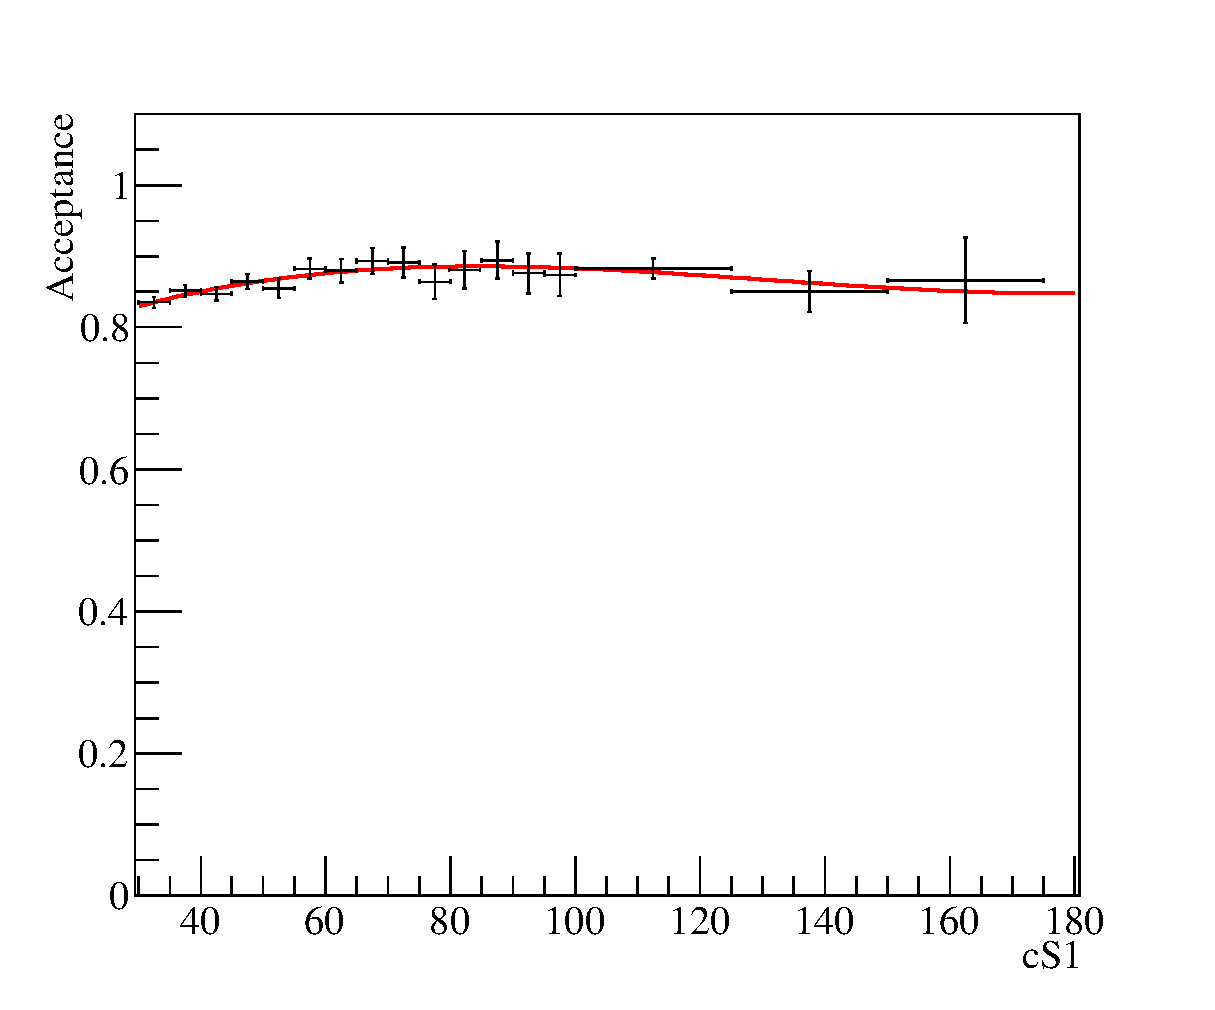
\includegraphics[width=1.\linewidth]{Figures/Acceptance.eps}}
\end{minipage}
\caption{The total acceptance of all cuts used, data from calibration in black and the fit in red.}
\label{fig:Acc}
\end{figure}

We define our signal region in the discrimination (y,cS1)-plane using $^{241}$AmBe calibration data. 
The ROI is shown in Figure~\ref{fig:phasespace} as blue contour lines: the upper bound is defined such that it is not contaminated from contribution due to xenon excitation lines, the lower is defined as the 3\,$\sigma$ acceptance quantile of the $^{241}$AmBe distribution.

We divide our signal region into two bands, they are constructed such that the $^{241}$AmBe data sample is equally distributed in y between them. The total number of events in a band is $\sim3000$ events. The bands are further divided into nine bins. The definition and content of the bins are presented in table~\ref{table:BinDef} and in Figure~\ref{fig:phasespace}. 


%%%%%%%%%%%%%%%%%%%%%%%%%%%%%%%%%%%%%%%%%%%%%%%%%%%%%%%%%%%%%%%%%%%%%%%%%%%%%%%%%%%%%%%%%%%%%%%%%%%%%%%

%%%%%%%% THIS PROBABLY NEEDS A SECTION, explaining well the uncertainty determination %%%%%%%%%%%%%%%%%
The main source of background results from  ER leakage and hence, we estimate the background distribution in the ROI using $^{60}$Co and $^{232}$Th calibration samples.  
Contribution from radiogenic and cosmogenic neutrons, and accidental coincidence are negligible for such a high energy recoil.
For illustration purposes we report in Table~\ref{table:BinDef} the background expectation for each ROI bin along side with the observed data events. The background expectation is computed by scaling the calibration sample yield by $6.54\times10^{-3}$, which is merely the ratio of observed data and calibration in an independent sideband. Note that in the background normalization is fitted to data during hypothesis testing, as described in section~\ref{sec:LikelihoodFunction}. 

%%%%%%%%%%%%%%%%%%%%%%%%%%%%%%%%%%%%%%%%%%%%%%%%%%%%%%%%%%%%%%%%%%%%%%%%%%%%%%%%%%%%%%%%%%%%%%%%%%%%%%%


\begin{table}
\resizebox{1.\columnwidth}{!}{

	 \begin{tabular}{|c| c| c| c| c| c |} 
 \hline
 \# & Band  & Energy Range (cS1)  & \# Background Events & \# Data Events \\  
 \hline\hline
 1 & upper & 30  - 40  & 23.5 & 20 \\ 
 \hline
 2 & upper & 40  - 50  & 15.7 & 17 \\
 \hline
 3 & upper & 50  - 80  & 12.4 & 11 \\
 \hline
 4 & upper & 80  - 120 & 1.1  & 1  \\
 \hline
 5 & upper & 120 - 150 & 0.1  & 1  \\  
 \hline
 6 & upper & 150 - 180 & 0.08 & 0  \\  
 \hline
 7 & lower & 30  - 50  & 0.9  & 0  \\  
 \hline
 8 & lower & 50  - 90 & 0.35 & 0  \\  
 \hline
 9 & lower & 120 - 180 & 0.18 & 0  \\  
 \hline
\end{tabular}
}

\caption{Bins definition. The estimated background event is calculated by taking the calibration sample and scaling it by $6.54\times10^{-3}$, which is the ratio of data and calibration in a sideband.}  \label{table:BinDef} 
\end{table}


\begin{figure}[]
\begin{minipage}{1\linewidth}
\centerline{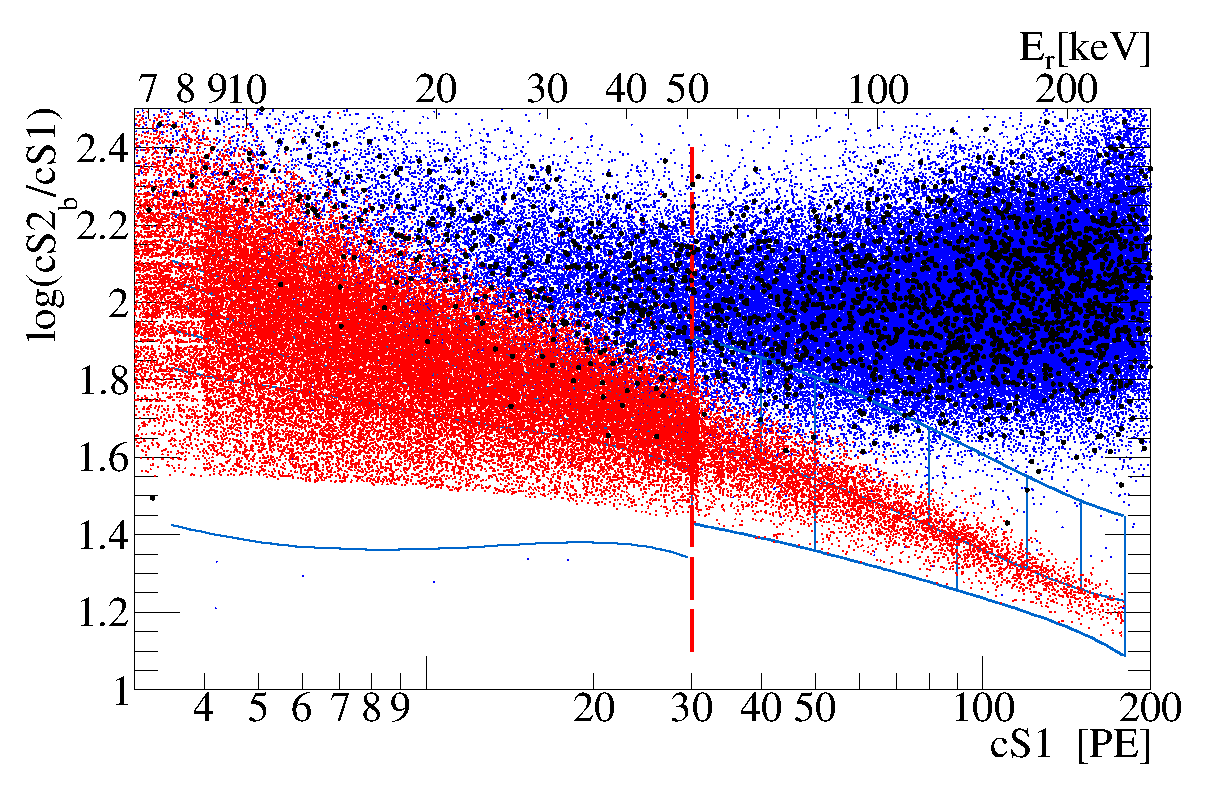
\includegraphics[width=1\linewidth]{Figures/eft_sr.eps}}
\end{minipage}
\caption{$^{60}\mathrm{Co}$ and $^{232}\mathrm{Th}$ data in light gray and DM data in black dots. The red line is the threshold between the lowE part and the highE one. In blue are the bands. For lowE constructed using data from a 50 GeV/$c^2$ WIMP. For the highE region the 9 bins are presented. top left is bin number 1,  top right is bin number 6, bottom left is bin number 7 and bottom right is bin number 9.}
\label{fig:phasespace}
\end{figure}  




\subsection{Signal Model}
\label{subsec:SignalModel}
The signal model is produced by taking a theoretical event rate spectrum, the production of which is described in sections \ref{subsubsec:Elastic} and \ref{subsubsec:Inelastic}, and applying the analysis acceptance and detector response as described in ~\cite{xe100_ana2012} (with modifications as stated above) to obtain the expected event rate in the detector in terms of detector variables (i.e. cS1,cS2). In order to calculate the expected value of the signal in cS1, we use Eq.~\ref{eq:LeffEnergyScale} for both energy regions, 
\begin{equation}
\label{eq:LeffEnergyScale}
	\langle cS1 \rangle = E_{\mathrm{nr}} \cdot (\Ly \Leff) \cdot   \left(\frac{S_{nr}}{S_{ee}}\right) 
\end{equation}
%\begin{multline}
%\label{eq:low2D}
%  \frac{\mathrm{d}^2 R}{\mathrm{d}\cSi.\mathrm{d}\cSiib} = \epsilon_\mathrm{S1}(\cSi).\epsilon_\mathrm{S2}(\cSiib) \\ 
%  \times \int \! \frac{\mathrm{d}R}{\mathrm{d}E}.p_\mathrm{S1}(\mathrm{\cSi}|E).p_\mathrm{S2}(\mathrm{\cSiib}|E) \, \mathrm{d}E
%\end{multline}

%where
%
%\begin{align}
%\label{eq:S1S2pdf}
% p_\mathrm{S1}(\mathrm{\cSi}|E) &= \sum_{N'} P_\mathrm{pmt}(\mathrm{\cSi}|N',0.5 \sqrt{N'}).\mathrm{Pois}(N'|\mu_\gamma) \\
% p_\mathrm{S2}(\mathrm{\cSiib}|E) &= \sum_{N'} P_\mathrm{pmt}(\mathrm{\cSiib}|Y N',\sigma_Y \sqrt{N'}).\mathrm{Pois}(N'|\mu_Q)
%\end{align}
%
%where $P_\mathrm{pmt}$ is a normal distribution with arguments as $N(x|\mu,\sigma)$, and where
%
%\begin{align}
%\mu_\gamma(E) &\approx E \cdot L_y \cdot L_\mathrm{eff}(E) \cdot \frac{S_\mathrm{nr}}{S_\mathrm{ee}} \\
%\mu_Q(E) &\approx Q_y(E) \cdot E
%\end{align}

where $E_\mathrm{nr}$ is the recoil energy, $\Ly$ is the light yield, $\Leff$ is the scintillation efficiency relative to 122$\keVee$ as a function of $E_\mathrm{nr}$, and $S_{ee}$ and $S_{nr}$ are the quenching factors for ER and NR respectively. Aside from $E_\mathrm{nr}$ and $\Leff$ these parameters have fixed values, namely $\Ly = 2.28$, $S_\mathrm{nr} = 0.95$, and $S_\mathrm{ee} = 0.58$. Recoils below 3 keV are assumed to produce no light since $\Leff$ is not measured at these energies. For details of the physics behind these parameters and the construction of the signal PDF please see \cite{xe100_ana2012,xe100_run_combination}. 

For the lowE region, the expected cS2 signal can be calculated as well~\cite{DataMCXenon} using Eq.~\ref{eq:Qy},
%
\begin{equation}
\label{eq:Qy}
	\langle cS2_{bottom} \rangle = E_{\mathrm{nr}}\Qy Y   
\end{equation}
%
where $Y = 8.4366$ is the amplification factor determined from the detector response to single electrons~\cite{XenonSingleElectron}, and $\Qy$ is the charge yield as a function of $E_\mathrm{nr}$. Note that as some of the top PMTs saturate we use only the bottom PMT for energy scale in S2. Applying the detector and PMT responses, and the acceptance as in \cite{xe100_run_combination}, defines the lowE signal model over the region $3 \mathrm{PE} < \cSi < 30 \mathrm{PE}$, with $\cSiib > 73.5 \mathrm{PE}$.

Eq. \ref{eq:Qy} hides a small subtlety. The actual $cS2_{bottom}$ PDF is composed of two pieces, a Poisson term associated with the initial charge liberation and a Gaussian term associated with the PMT response and other detector effects:
%
\begin{equation}
\label{eq.cS2pdf}
p_\mathrm{S2}(\mathrm{\cSiib}|E) = \sum_{N'} P_\mathrm{pmt}(\mathrm{\cSiib}|Y N',\sigma_Y \sqrt{N'}).\mathrm{Pois}(N'|\mu_Q)
\end{equation}
%
where $\mu_Q=E_{\mathrm{nr}}\Qy$ is the expected number of liberated charges in a nuclear recoil event of energy $E$, and $N'$ is the actual number of liberated charges, which are unmeasured and thus summed over. The amplification factor $Y$ is applied on the actual number of liberated charges $N'$, not the expected number $\mu_Q$. Associated with this is the variance of the Gaussian response PDF, $\sigma_Y\sqrt{N'}$, where in this analysis $\sigma_Y = 6.93$. 

For the high energy region we can not produce the S2 distribution as the method in~\cite{DataMCXenon} is not calibrated for high enough recoil energies. We therefore use the NR calibration data distribution in log($\mathrm{cS2_b/cS1}$) to estimate the WIMP one. Above 180PE in \cSi\ the statistics of $^{241}$AmBe data is too low to estimate the distribution accurately so this forms the higher bound of this analysis. With the \cSiib\ distribution determined by this empirical method we require only a prediction of the \cSi\ distribution. This is obtain from Eq. \ref{eq:LeffEnergyScale}, followed by the application of detector and PMT responses, as well as the acceptance given in~\ref{fig:Acc}, which completes the highE signal model definition.

Examples of each for two EFT operators are shown in Figures ~\ref{fig:HighE} and \ref{fig:LowE}, with the rate normalized to give 5 events in the total energy range (lowE and highE).

\begin{figure}[h!]
\begin{minipage}{1.\linewidth}
\centerline{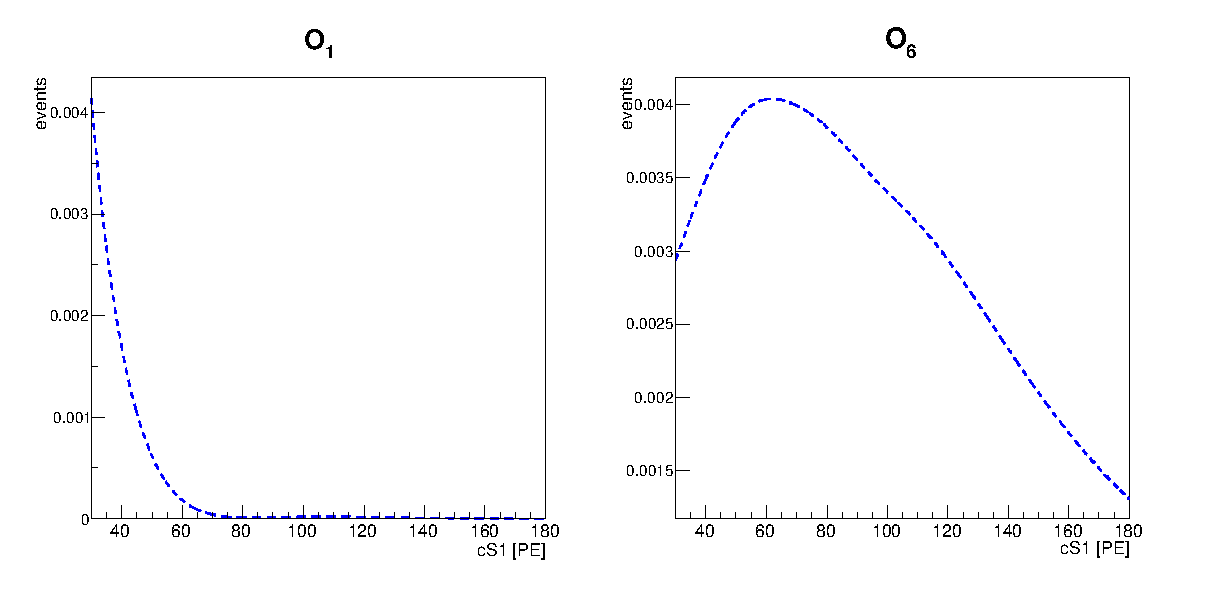
\includegraphics[width=1.\linewidth]{Figures/SigHighO1O6.eps}}
\end{minipage}
\caption{The expected signal in the high energy region for a 300 GeV/$c^2$ WIMP mass, Normalized to 5 events. Left(right) is the spectra for $O_1$($O_6$). Notice that for $O_1$ most of the events are not expected to deposit energy higher then 30 PE whereas for $O_6$ a large fraction of the events appear in this region.}
\label{fig:HighE}
\end{figure} 

\begin{figure}[h!]
\begin{minipage}{1.\linewidth}
\centerline{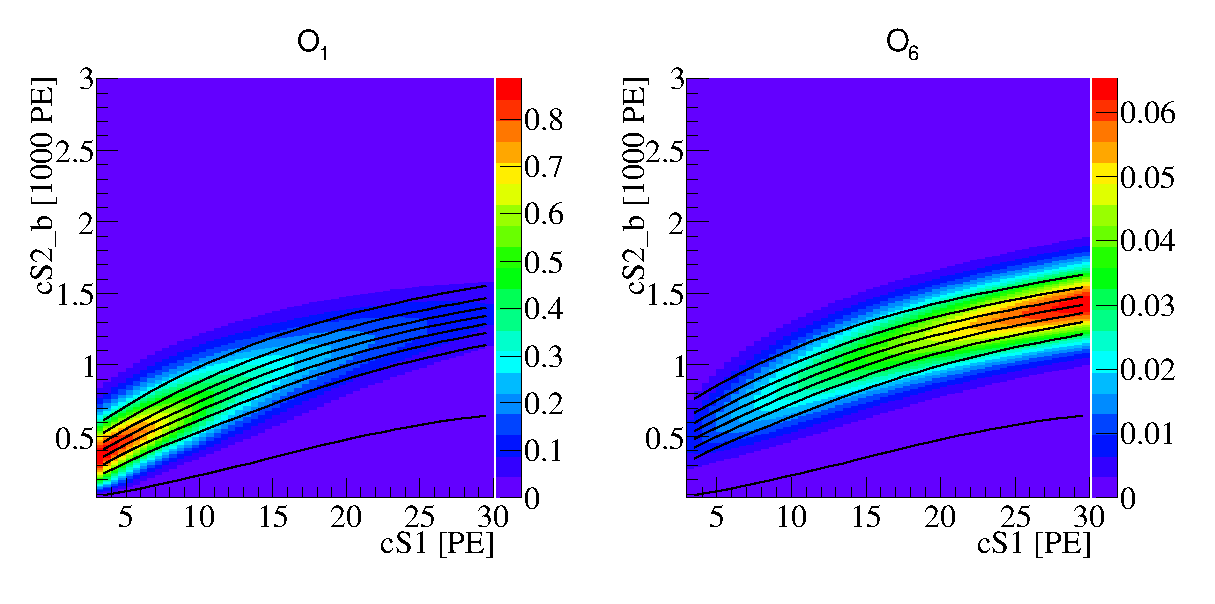
\includegraphics[width=1.\linewidth]{Figures/SigLowO1O6.eps}}
\end{minipage}
\caption{The expected signal in the low energy region for a 300 GeV/$c^2$ WIMP mass, Normalized to 5 events. Left(right) is the spectra for $\mathcal{O}_1$($\mathcal{O}_6$). Notice that for $\mathcal{O}_1$ most of the events are expected to deposit energy lower then 30 PE whereas for $\mathcal{O}_6$ a large fraction of the events do not appear in this region at all. The black lines indicate the bands constructed on this specific event rate, and are dividing the signal into 8 equally distributed signal sub-regions.}
\label{fig:LowE}
\end{figure}




%
%\begin{multline}
%\label{eq:high2D}
%  \frac{\mathrm{d} R}{\mathrm{d}\cSi} = \epsilon_\mathrm{S1}(\cSi) \int \! \frac{\mathrm{d}R}{\mathrm{d}E}.\epsilon_\mathrm{S2'}(E).p_\mathrm{S1}(\mathrm{\cSi}|E) \, \mathrm{d}E
%\end{multline}

%\sout{
%where $p_\mathrm{S1}(\mathrm{\cSi}|E)$ is computed as in Eq. \ref{eq:S1S2pdf}. The S1 acceptance $\epsilon_\mathrm{S1}(\cSi)$ is given in Fig. \ref{fig:Acc}, and the S2 acceptance $\epsilon_\mathrm{S2'}(E)$ is negligibly different from one over the signal region $30 \mathrm{PE} < \cSi < 180 \mathrm{PE}$.
%}
\subsubsection{Elastic Scattering}
\label{subsubsec:Elastic}

The expected recoil energy spectrum of each WIMP mass for each EFT operator is calculated using the Mathematica package \texttt{DMFormFactor} supplied by Anand et. al.~\cite{Fitzpatrick:MathTools,Anand:MathTools}. We use standard assumptions as in previous analyses (e.g \cite{xe100_run_combination}) regarding the local dark matter density and velocity distribution, namely $\rho_\mathrm{local} = 0.3$ GeV/cm\textsuperscript{3} and a Maxwell-Boltzman distribution with a mean given by the local circular velocity $v_0 = 220$ km/s and cut off at an escape velocity of $v_\mathrm{esc} = 544$ km/s. The responses of Xe nuclei to a scattering event are computed from one-body density matrices provided with the package, in contrast to the Helm form factors which have been used in previous analyses. These spectra are produced for the seven most abundant Xe isotopes (128,129,130,131,132,134 and 136), combined in proportion to the abundance of these isotopes in the experiment \cite{xe100_run10_sd}, then translated into expected signal rates via the method described above.

\subsubsection{Inelastic WIMP Scattering}
\label{subsubsec:Inelastic}
\RanComment{We should add here the dependency of $v_{min}$ on $\delta$}
To obtain recoil spectra for WIMP-nucleon scattering for all EFT operators with inelastic kinematics, we use a modified version of \texttt{DMFormFactor} provided by Barello et. al. \cite{InelasticMath}. Assumptions regarding the dark matter halo and nuclear physics are unchanged. The mass splitting $\delta$ between dark matter states is varied from 0 to \sout{1000} \RanComment{300} keV, \sout{well} beyond the value at which the predicted rate is zero for the entire mass range we consider (\RanComment{we see nothing above 250keV mass splitting}) \BenComment{perhaps I should see what number that actually is}.
